\section{Multi-Regime Results}
\label{sec:results}

This work evaluates machine-unlearning robustness under four primary recovery-radius regimes: strong per-example conditional recovery, conditional patches, border-frame delivery, and multi-patch local delivery. Across the main benchmark rows audited in depth---SalUn, SCRUB, RURK, CE-U, BalDRO, and ORBIT---the dominant threat remains targeted per-example recovery, while universal perturbations are mostly ineffective on the stronger checkpoints. The point of this matched audit is not to ask whether a target-class adversarial perturbation exists in the abstract. It is to ask whether forget examples are selectively easier to drive back to the forgotten class than matched retain controls. Figure~\ref{fig:subspace-tradeoff} and Table~\ref{tab:subspace-defense} summarize the main defense result: feature-subspace stage-2 gives positive point-estimate shifts on BalDRO, SalUn, and ORBIT without collapsing clean accuracy, with the clearest practical signal on ORBIT and SalUn and only a tiny BalDRO shift. Figure~\ref{fig:robust-frontier} shows that robust-base SalUn does not eliminate leakage outright; instead it moves along a utility-vs-recovery frontier. Figure~\ref{fig:patch-regime} shows that conditional patches remain viable, but only for a subset of methods.

\begin{table}[t]
  \centering
  \small
  \setlength{\tabcolsep}{3pt}
  \begin{tabular}{l l c c c}
    \toprule
    Model & Setup & Forget Median$^\ast$ & Retain Median$^\ast$ & Clean Forget Rate \\
    \midrule
    BalDRO$^\S$ & baseline & 0.00343 & 0.00846 & 0.000 \\
    BalDRO$^\S$ & feature-subspace stage-2 & 0.00349 & 0.00858 & 0.000 \\
    SalUn & baseline & 0.00251 & 0.00564 & 0.031 \\
    SalUn & feature-subspace stage-2 & 0.00276 & 0.00600 & 0.031 \\
    ORBIT & baseline & 0.00340 & 0.00643 & 0.031 \\
    ORBIT & feature-subspace stage-2 & 0.00423 & 0.00690 & 0.000 \\
    RURK$^\S$ & baseline & 0.00159 & 0.00576 & 0.062 \\
    RURK$^\S$ & feature-subspace stage-2 & 0.00159 & 0.00576 & 0.062 \\
    CE-U$^{\dagger\S}$ & baseline & 0.00368 & ---$^\ddagger$ & 0.000 \\
    SCRUB & baseline only & 0.01078 & 0.00980 & 0.000 \\
    \bottomrule
    \multicolumn{5}{p{0.92\linewidth}}{\footnotesize $^\ast$Finite-success medians, not censored all-sample medians; recovery rates and censoring are tracked in the JSON artifacts.}\\
    \multicolumn{5}{p{0.92\linewidth}}{\footnotesize $^\dagger$CE-U: 2-step pilot audit, $n{=}8$, seed 42.}\\
    \multicolumn{5}{p{0.92\linewidth}}{\footnotesize $^\ddagger$0 of 8 retain-control attacks succeeded within $\epsilon$; finite-success retain median undefined.}\\
    \multicolumn{5}{p{0.92\linewidth}}{\footnotesize $^\S$Objective-level adaptation, not a faithful reproduction: BalDRO-\emph{style} softmax reweighting, RURK-\emph{style} random-noise robustness, and CE-\emph{ascent} (labeled CE-U). See Table~\ref{tab:method-classification} and Appendix~\ref{sec:adaptation}.}\\
  \end{tabular}
  \caption{Finite-success recovery-radius medians under the strongest per-example conditional attack. Feature-subspace stage-2 gives positive point-estimate shifts for BalDRO, SalUn, and ORBIT, but this table should not be read as a significance table: BalDRO's shift is tiny, and the available stage-2 rows are not fully seed-paired against every baseline. RURK and CE-U are flat under this full-image defense family; SCRUB is a seed-sensitive negative control with nearly identical forget and retain radii on most seeds. CE-U retains 0 of 8 retain-control attacks in the pilot audit, which is suggestive but not statistically comparable to the full-audit rows. Rows use $n=32$ samples per class per seed where available, except where noted. The distributed SalUn baseline checkpoint does not reproduce its reported row; regenerated 3-seed SalUn baseline numbers are in the reproducibility appendix.}
  \label{tab:subspace-defense}
\end{table}

\begin{figure}[t]
  \centering
  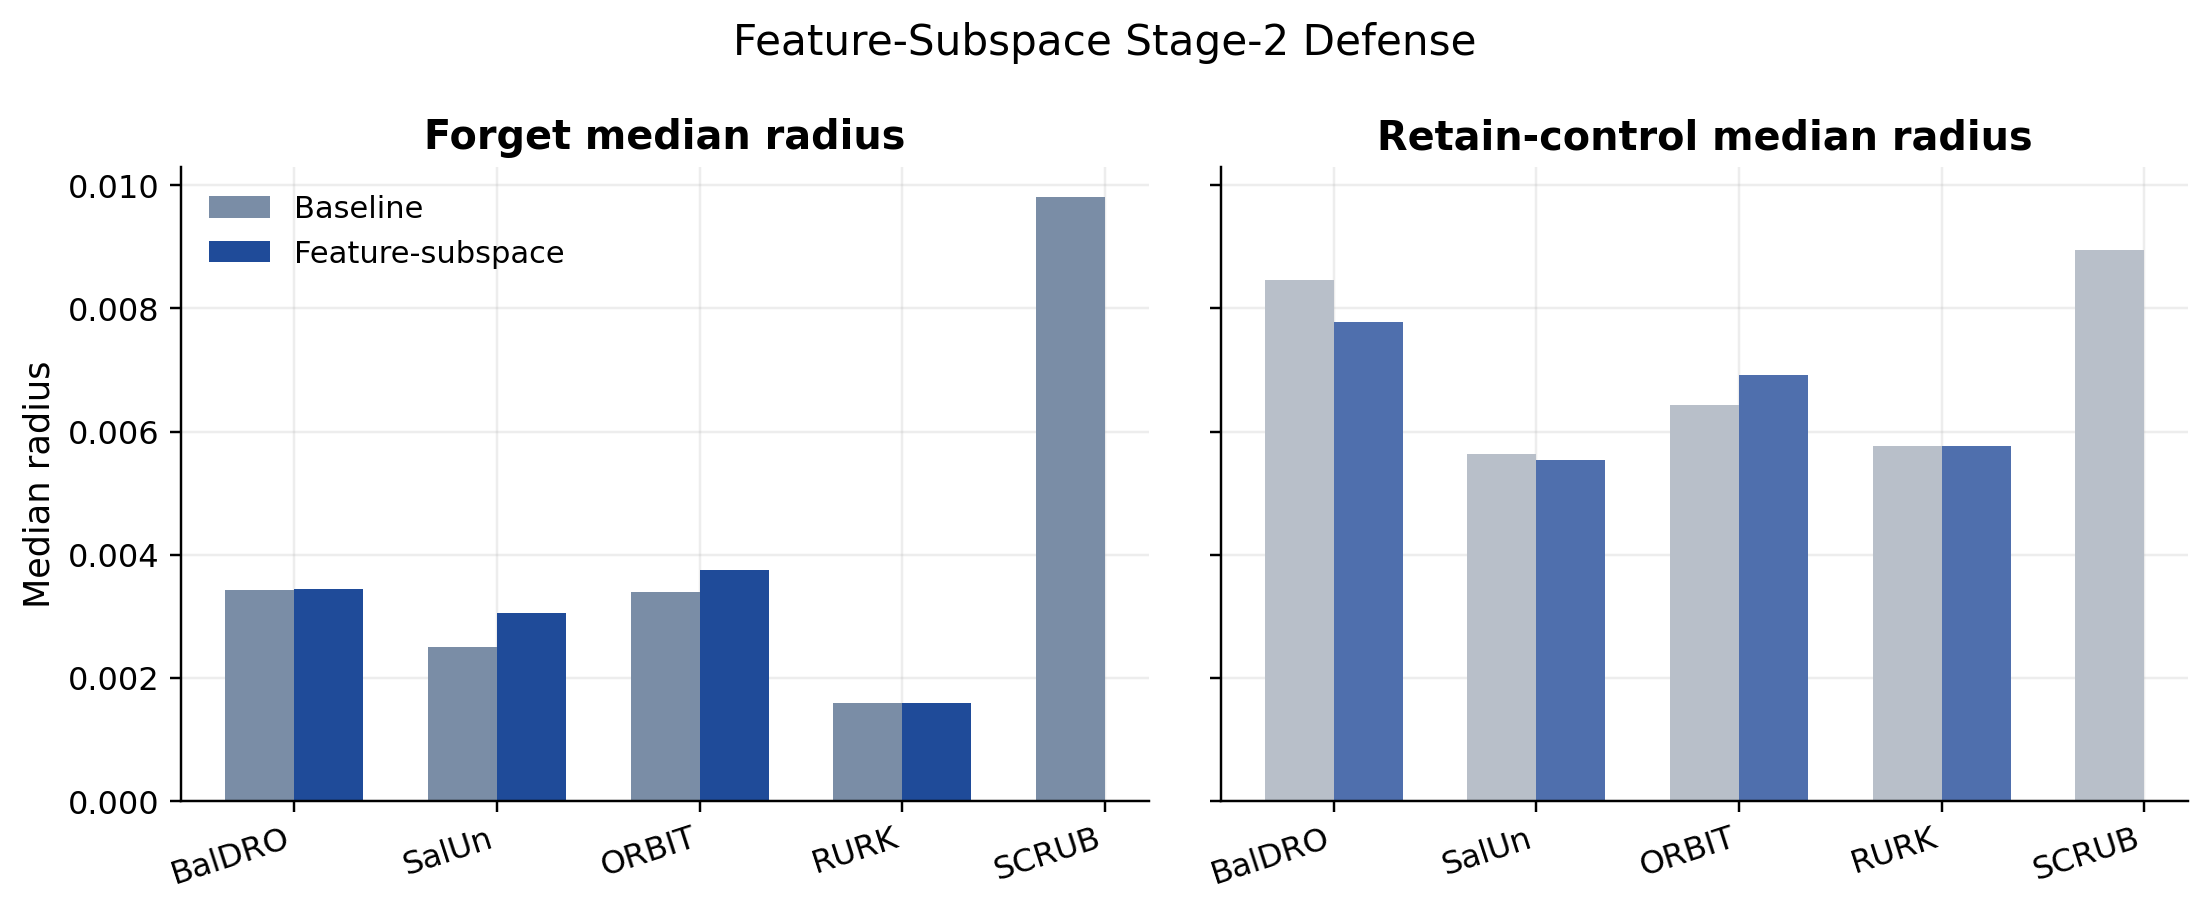
\includegraphics[width=0.92\linewidth]{feature_subspace_tradeoff.png}
  \caption{Feature-subspace stage-2 tradeoff. Larger forget medians indicate stronger resistance to conditional recovery. The plotted point estimates improve most clearly on ORBIT and SalUn, shift only slightly on BalDRO, and do not move RURK. Controlled paired confidence intervals require re-auditing matched-attack baselines from reproducible checkpoints and remain future work.}
\label{fig:subspace-tradeoff}
\end{figure}

\paragraph{Feature-subspace stage-2 defense.}
The most promising post-hoc defense family in the current benchmark is a feature-subspace stage-2 finetune. Rather than modifying the entire forgetting objective from epoch 0, the defense begins from an already-unlearned adapter and suppresses attacked forget-sample features inside a learned recovery subspace. This regime avoids the instability of earlier logit-margin defenses and produces positive point-estimate shifts on BalDRO, SalUn, and ORBIT. The effect is clearest on ORBIT and SalUn; the BalDRO shift is numerically tiny, and the table does not yet include the paired confidence intervals needed to treat it as statistically established. The effect is modest in absolute magnitude because the benchmark is CIFAR-10 under an $L_\infty$ budget on 224$\times$224 inputs, where successful radii are numerically small by construction. What matters in the current evidence is that some rows shift the forget-vs-retain frontier in the right direction without sacrificing clean retain utility, not that feature-subspace training is a universal defense.

\paragraph{CE-U as a core baseline.}
CE-U belongs in the main benchmark even though its first qualified positive defense row appears in the patch regime rather than under full-image recovery. Under the 2-step pilot audit (n=8, seed 42), the baseline CE-U checkpoint has forget median 0.00368 with 0\% clean forget success, and retain-control attacks succeed 0 of 8 times within the $\epsilon$ budget. This is suggestive pilot evidence for selectivity, but it is not ranked against SalUn or ORBIT because those rows use larger full audits. CE-U full-image feature-subspace stage-2 variants are at best flat, and the combined row is slightly worse under the APGD cross-check, so the CE-U defense claim is reserved for the qualified combined stage-2 patch result discussed below.

\begin{figure}[t]
  \centering
  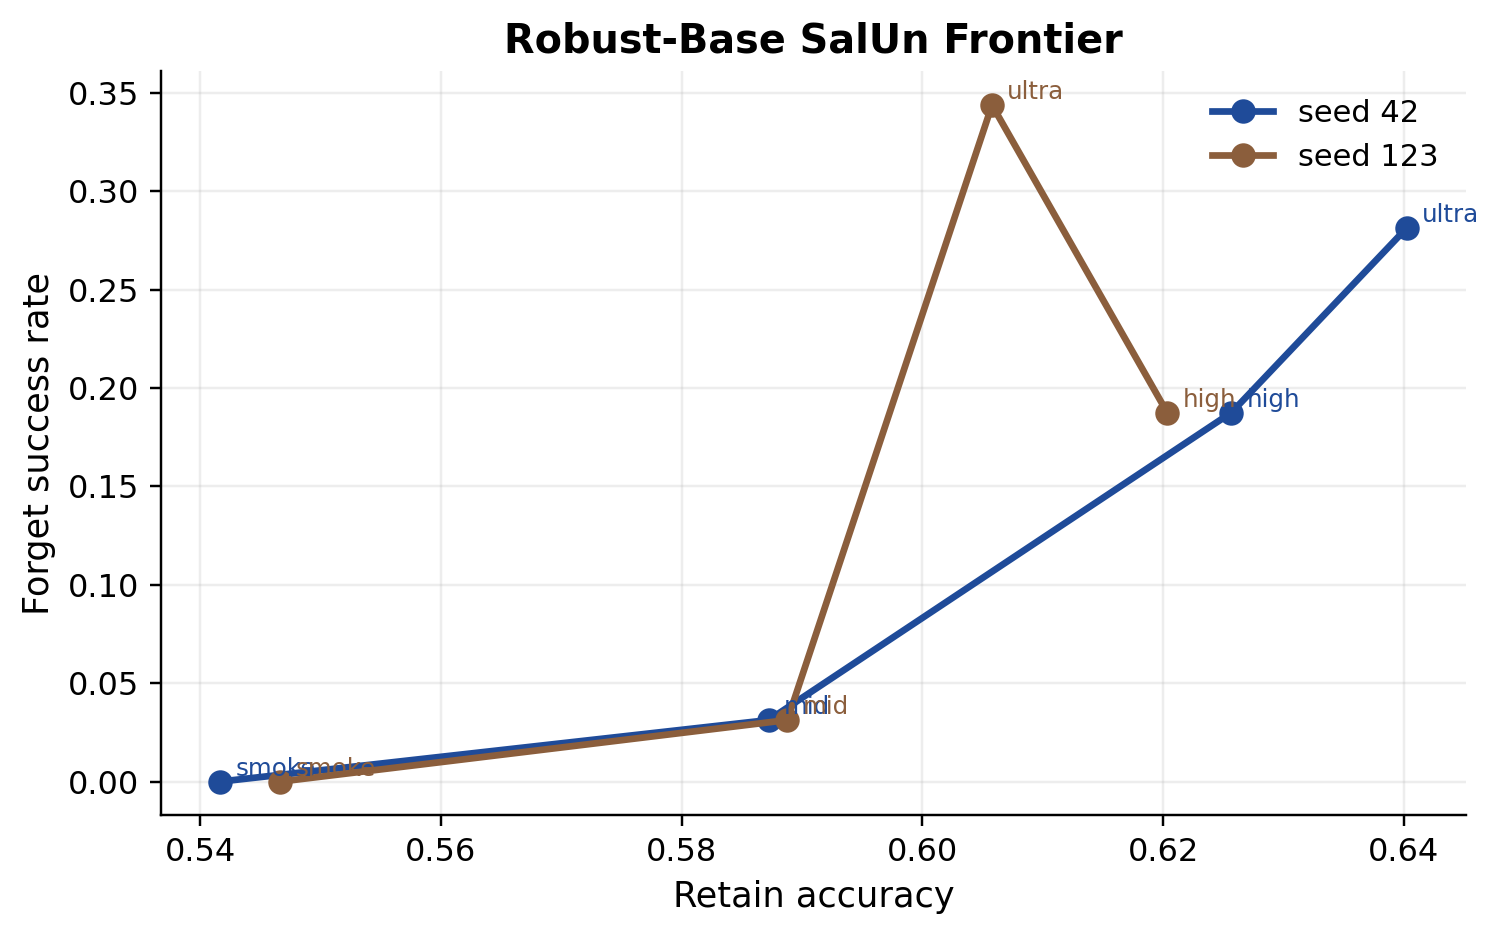
\includegraphics[width=0.92\linewidth]{robust_base_frontier.png}
  \caption{Robust-base SalUn frontier. Lower-utility robust-base checkpoints suppress conditional recovery more strongly, but leakage returns as retain utility improves.}
  \label{fig:robust-frontier}
\end{figure}

\paragraph{Robust-base frontier.}
Robust-base SalUn does not behave like a binary defense success. Instead, it exposes a frontier: at low utility, conditional recovery can drop to zero on the sampled audit; as retain accuracy rises, recovery reappears. This is a stronger framing than a single checkpoint claim because it shows that robustness and post-unlearning utility are coupled. Robust-base training is therefore treated as an operating-point choice rather than a one-shot fix.

\begin{figure}[t]
  \centering
  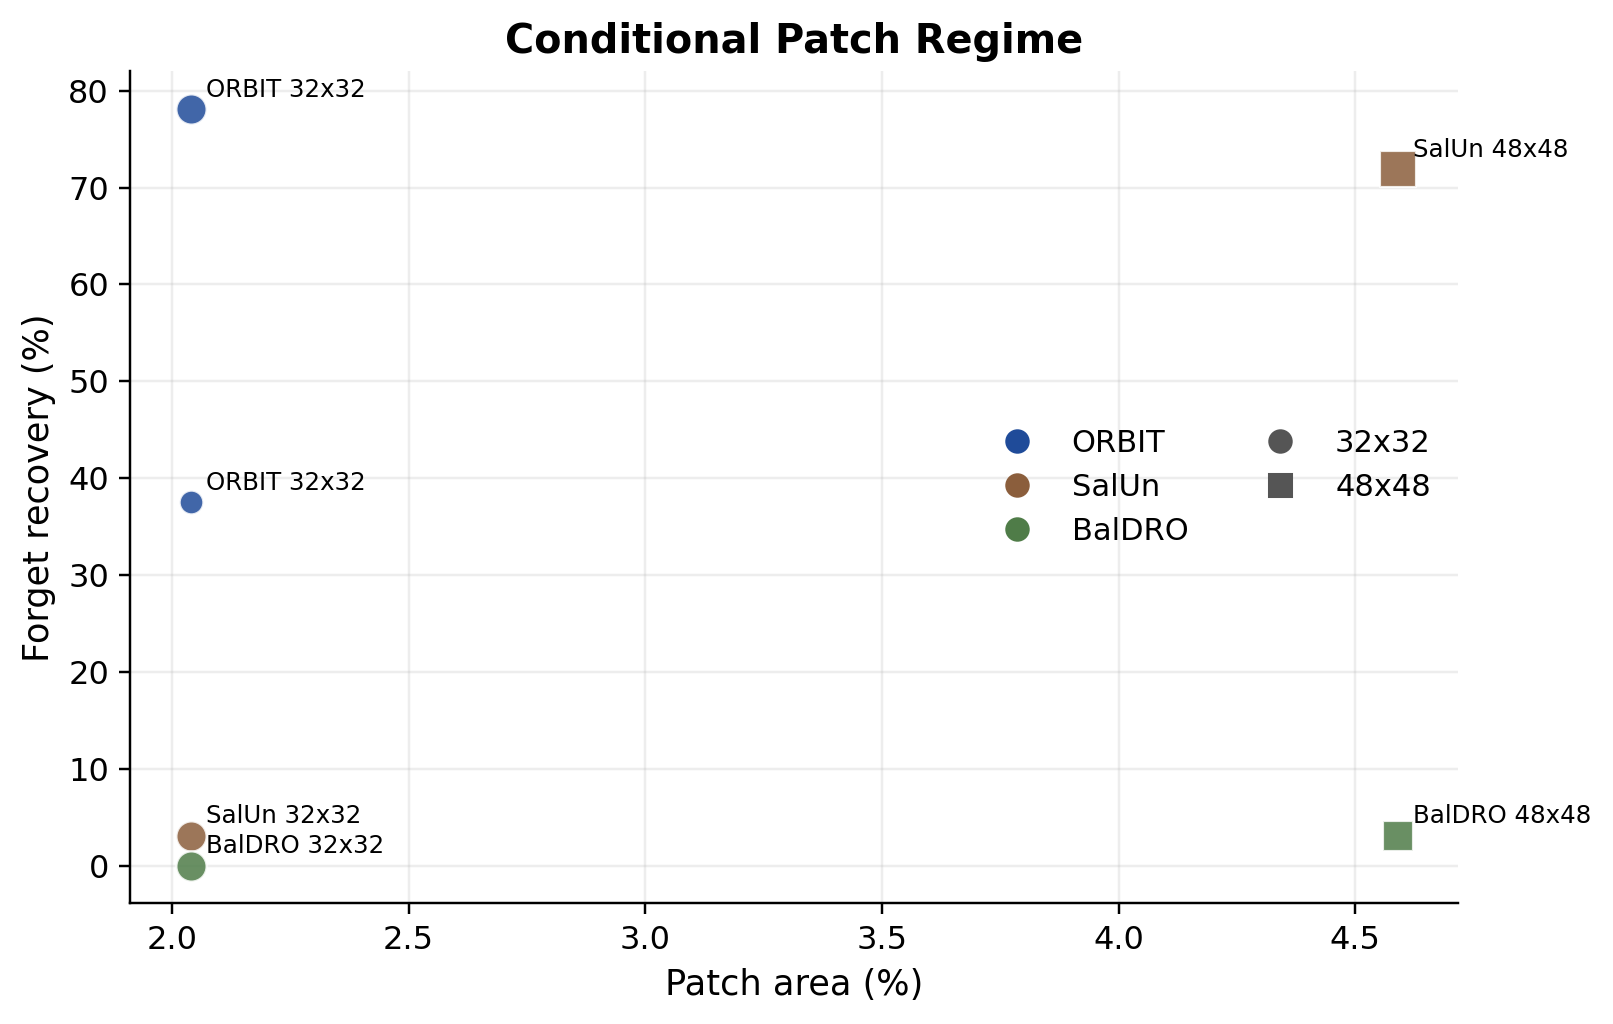
\includegraphics[width=0.92\linewidth]{conditional_patch_regime.png}
  \caption{Conditional patch regime. ORBIT admits strong low-area patch recovery, SalUn requires a larger patch and incurs more retain damage, and BalDRO is effectively negative under the same patch family.}
  \label{fig:patch-regime}
\end{figure}

\paragraph{Conditional patches.}
The patch result is not a universal trigger. Universal static patches were mostly ineffective on the stronger methods. The viable regime is instead a conditional small-area patch attack whose content and placement depend on the input. ORBIT is the flagship positive case: a 32$\times$32 patch covering 2.04\% of the image recovers forgotten behavior strongly while inducing no retain-to-forget hijack. SalUn is patch-vulnerable only at a larger 48$\times$48 budget, and BalDRO is effectively negative at both tested patch sizes. This method dependence reinforces the broader paper thesis: residual forgetting leakage is structured, but not universal.

\paragraph{Delivery surfaces beyond one patch.}
The later delivery-surface checks strengthen the attack story and narrow the defense story. Conditional frame attacks and conditional multi-patch attacks are both real local delivery surfaces, but they do not behave like simple extensions of the one-patch regime. Patch-aware defenses that help on one square patch often fail to transfer: the ORBIT patch-stage2 row becomes easier to recover under the frame attack, CE-U combined stage-2 also becomes easier and adds retain-side failure under the frame attack, and faithful full-ft SalUn patch-stage2 becomes easier under multi-patch delivery. The main exception is weak positive transfer from the ORBIT patch-stage2 row to multi-patch delivery. Frame and multi-patch regimes are therefore treated as first-class red-team surfaces rather than appendix-only perturbation variants.

\paragraph{Second-wave defenses.}
Two later branches sharpen the story. First, teacher-guided stochastic CVaR provides a small but reproducible full-image defense improvement on ORBIT across two seeds, whereas the same probabilistic family remains neutral on CE-U. Second, a combined subspace-plus-patch stage-2 defense gives the first CE-U row that improves under matched Adam audits while also reducing conditional patch success, although its APGD result is still slightly worse than baseline. By contrast, the larger mixed-surface stage-2 defense was explicitly designed to transfer across one-patch, frame, and multi-patch delivery and failed to do so reliably. These later rows are therefore useful but qualified: they extend the defense story beyond pure feature-subspace training without becoming universal fixes.

\paragraph{Takeaway.}
The combined evidence supports a multi-regime view of red-teaming machine unlearning. Strong per-example conditional attacks remain the main threat, conditional patches expose an additional local attack surface on some methods, and frame plus multi-patch attacks show that local-delivery robustness is materially harder than one-patch robustness alone. The best defense families found here are modest and method-specific: feature-subspace stage-2 gives the clearest point-estimate gains on ORBIT and SalUn, teacher-guided stochastic CVaR helps ORBIT slightly, and CE-U combined stage-2 is only a qualified partial row. RURK remains a hard case, and SCRUB serves as a seed-sensitive negative control where generic adversarial fragility usually overwhelms forget-specific interpretation.
